\chapter{Visualização simultânea de imagens e superfície}

A visualização simultânea de imagens e superfície pode ser acionada clicando com o botão
\textbf{esquerdo} do mouse sobre o atalho localizado no canto inferior direito da tela do
InVesalius. Veja a figura \ref{fig:slice_plane_original}.

\begin{figure}[!htb]
\centering
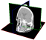
\includegraphics[scale=0.6]{../user_guide_figures/icons/slice_plane_original.png}
\caption{Atalho para visualização simultânea}
\label{fig:slice_plane_original}
\end{figure}

Este recurso permite habilitar ou desabilitar a exibição das imagens nas diferentes
orientações (ou planos) na mesma janela de visualização da superfície 3D. Para isso, basta
marcar ou desmarcar a opção correspondente no menu indicado na figura \ref{fig:view_2d_3d_1}.

\begin{figure}[!htb]
\centering
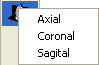
\includegraphics[scale=0.6]{../user_guide_figures/invesalius_screen/view_2d_3d_1.png}
\caption{Seleção das orientações (planos) a exibir}
\label{fig:view_2d_3d_1}
\end{figure}

Vale notar que uma orientação, quando selecionada, apresenta uma marca na opção correspondente.
Isso é ilustrado na figura \ref{fig:view_2d_3d_2}.

\begin{figure}[!htb]
\centering
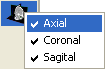
\includegraphics[scale=0.6]{../user_guide_figures/invesalius_screen/view_2d_3d_2.png}
\caption{Orientações selecionados para exibição}
\label{fig:view_2d_3d_2}
\end{figure}


\newpage


Se a superfície já estiver sendo exibida, os planos das orientações serão apresentados como mostra
a figura \ref{fig:3d_planes}. Caso contrário, somente os planos serão exibidos
(figura \ref{fig:only_2d_planes}).

\begin{figure}[!htb]
\centering
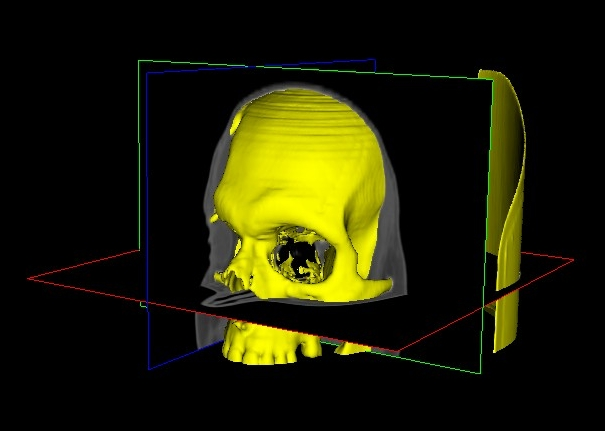
\includegraphics[scale=0.5]{../user_guide_figures/invesalius_screen/3d_planes.jpg}
\caption{Superfície e planos exibidos simultaneamente}
\label{fig:3d_planes}
\end{figure}

\begin{figure}[!htb]
\centering
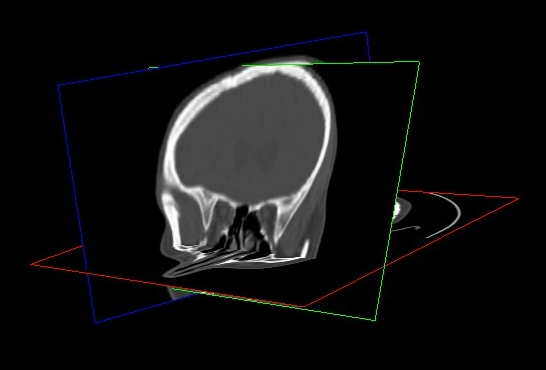
\includegraphics[scale=0.55]{../user_guide_figures/invesalius_screen/only_2d_planes.jpg}
\caption{Exibição de planos (sem superfície)}
\label{fig:only_2d_planes}
\end{figure}

\newpage

Para desativar a exibição de um plano, basta desmarcar a opção correspondente no menu
(figura \ref{fig:view_2d_3d_2}).
